\chapter{Knowledge-driven Acoustic Echo Retrieval \& \blaster}\label{chap:blaster}

\marginpar{%
\footnotesize
\textbf{Keywords:} Blind Channel Identification, Super Resolution, Sparsity, Acoustic Impulse Response.
}
\newthought{Synopsis} Acoustic echoes retrieval is a research topic that is gaining importance in many speech and audio signal processing applications
such as speech enhancement, source separation, dereverberation and room geometry estimation.
This work proposes a novel approach to blindly retrieve the \textit{off-grid} timing of early acoustic echoes %\textit{i.e.},
from a stereophonic recording of an unknown sound source such as speech. It builds on the recent framework of continuous dictionaries.
In contrast with existing methods, the proposed approach does not rely on parameter tuning nor peak picking techniques by working directly in the parameter space of interest.
The accuracy and robustness of the method are assessed on challenging simulated setups with varying noise and reverberation levels and are compared to two state-of-the-art methods.

\section{Introduction}
\label{sec:blaster:intro}
%Striking introducing sentence
In room acoustics and audio signal processing, the temporal structure of the room impulse response (RIR) plays a central role.
% First echo is noise
It is the result of multiple (indirect) sound propagation paths due to specular and diffuse reflections on the room's surfaces, leading to reverberation~\cite{Wang2011}.
In such conditions, the perceived sound quality is often considered degraded and it is common to observe a detrimental decrease of performance as reverberation increases for applications such as speech recognition~\cite{Yoshoka2012} or music information retrieval~\cite{Barthet2010}.
% or music virtual reality~\cite{DeMan2017}. %to observe a detrimental decrease of performances with reverberation. as well as music virtual reality~\cite{DeMan2017}.
%\textcolor{red}{Add something about amazon echo, google assistant (analysis) and virtual reality (rendering/synthesis)}

% Second echo is information
On the other hand, RIRs contain very rich geometrical information about the acoustic scene.
%which is independent from the source signal itself.
%In contrast with well-consolidated methods,
Recent \textit{echo-aware} works have shown that the knowledge of the timing of early reflections may boost performance in many audio signal processing applications,
from dereverberation~\cite{Wu2006,Lin2008} to sound localization~\cite{Ribeiro2010,DiCarlo2019} and separation~\cite{Dokmanic2015a, Scheibler2017}.
Moreover, it allows joint estimation of the receivers' positions~\cite{Salvati2016}, the reflective surfaces~\cite{Antonacci2012} and consequently the geometry of the room~\cite{Dokmanic2013, Crocco2017}.
% or acoustic impedance of surfaces~\cite{Antonello2014, Bertin2016}.
% beamforming \cite{Dockmanic2015},
% such as for speech enhancement \cite{Wu2006}, source localization \cite{Ribeiro2010}, source separation \cite{Scheibler2017} and dereverberation \cite{Lin2009}
% which are common pre-processing steps for many applications \cite{Gannot2017}

Acoustic echo retrieval (AER) consists in estimating the properties of the early (strong) acoustic reflections only in
multi-path environments~\cite{Tukuljac2018}, sometimes referred to as time delay estimation~\cite{Chen2006a}.
To achieve this, several methods rely on a known source signal~\cite{park2017compressive,jensen2019method}.
% Adding unknown adds a line :-(
% yes, but it is really important
% Got it. New mission: win space somewhere else in the paragraph?
% no problem, I will pass throughthhtghththghth this
% Seems legit
In contrast, when multiple receivers attend an unknown single source, AER can be seen as an instance of Single Input Multiple Output (Blind) Channel Estimation (SIMO-BCE) problem.
%or \textit{system identification}, \textit{i.e.} estimating the filters entailing an unknown input observed output of a system.
%In a more challenging setting, when no prior information about the source signal are available, the problem is referred to as SIMO \textit{blind channel estimation} (SIMO-BCE) \cite{Lin2007}.
A common approach for solving AER in the context of SIMO-BCE is to first blindly estimate a discrete version of the acoustic channels using the so-called cross-relation identity~\cite{Xu1995, Crocco2016}.
The location of the echoes are then chosen among the strongest peaks with ad-hoc peak-picking techniques.
%Such methods are generally \emph{on-grid} in the sense that the estimation relies on a fixed grid of points and \textit{a priori} chosen filter lengths.
However, in practice, the true timings of echoes rarely match the sampling grid, thus leading to pathological issues called basis-mismatch in the field of compressed sensing.
To circumvent this issue, the authors of~\cite{Tukuljac2018} proposed to leverage the framework of finite-rate-of-innovation sampling to make one step towards off-grid approaches.
Despite promising results in the absence of noise and with synthetic data, the quality of the estimation highly relies on an initialization point.

Of particular interest in this paper is the recently proposed framework of continuous dictionaries (CD)~\cite{Carlos2014}.
By formulating an inverse problem as the recovery of a discrete measure over some parameter space, CD has allowed to overcome imaging device limitations in many applications such as super-resolution~\cite{Carlos2014} or PALM/STORM imaging~\cite{denoyelle2019}.
In this work, we formulate the problem of stereo AER within the framework of continuous dictionaries.
The resulting optimization problem is convex and thus not prone to spurious minimizers.
The proposed method is coined \emph{Blind And Sparse Technique for Echo Retrieval} (\blaster) and requires no parameter tuning.
The method is compared to state-of-the art on-grid approaches under various noise and reverberation levels using simulated data.
While comparable or slightly worse recovery rates are observed for the task of recovering 7 echoes or more, better results are obtained for fewer echoes and the off-grid nature of the approach yields generally smaller estimation errors.


\section{Background in Acoustic Echo Estimation}
\label{sec:blaster:background}

\subsection{Signal and measurement model}
Consider the common setup where a band-limited and square-integrable source signal $\contSource$ is emitted.
Due to the geometry of the room, the latter signal is both reflected (several times) and attenuated before reaching a set of two microphones.
The recorded signal at microphone $i\in\{1,2\}$ reads
\begin{equation}
    \label{eq:recordedSignal}
    \contRecordedSignal_i = \contSource \ast \contFilter_i^\star + \contNoise_i
\end{equation}
where $\ast$ denotes the (continuous) convolution operator, $\contNoise_i$ models some additive noise in the measurement process and $\contFilter_i^\star$ denotes the room impulse response (RIR).
In the remainder of this paper, the  superscript $\star$ refers to the ground truth.
In AER, we are interested in RIRs that are streams of Diracs, \textit{i.e.},
\begin{equation}
    \label{eq:def_filter_star}
    \contFilter_i^\star(t) = \sum_{r=0}^{R_i-1} c_{i,r} \delta(t - \tau_{i,r})
\end{equation}
where $R_i$ is the (unknown) number of echoes, $\kfamily{\tau_{i,r}}{r=0}^{R_i-1}$ models the echoes' delays, and $\kfamily{c_{i,r}}{r=0}^{R_i-1}$ are the corresponding non-negative attenuations.
Note that $r=0$ defines the direct propagation path.
%
In the noiseless case, that is when $\contNoise_i=0$ for $i\in\{1,2\}$, we have the identity
\begin{equation} \label{eq:cross-relation}
    \contRecordedSignal_1 \ast \contFilter_2^\star = \contRecordedSignal_2 \ast \contFilter_1^\star
\end{equation}
by commutativity of the convolution operator.
This result is dubbed cross-relation identity in the channel identification literature \cite{Xu1995}.
Hence, one can expect to recover the two filters by solving an optimization problem involving~\eqref{eq:cross-relation}.
%the difference between the two terms in~\eqref{eq:cross-relation}.

However, in practice, only sampled versions of the two recorded signals are available.
More precisely, we consider a  measurement model where the incoming signal undergoes a (ideal) low-pass filter $\idealLowPassFilter$ with frequency support $\kintervcc{\sfrac{-\Fs}{2}}{\sfrac{\Fs}{2}}$ before being regularly sampled at the rate  $\Fs$.
We denote $\disRecordedSignal_1,\disRecordedSignal_2\in\kR^{2N}$ the two vectors of $2N$ (consecutive) samples and $i\in\{1, 2\}$ by
\begin{equation}
    \label{eq:measurement-process}
    \disRecordedSignal_i[n] =
    \kparen{\idealLowPassFilter \ast \contRecordedSignal}\kparen{\frac{n}{\Fs}}
    \qquad
    \forall n \in\{0, \dots, 2N-1\}
    .
\end{equation}
%Let $\disRecordedSignal_1,\disRecordedSignal_2\in\kR^N$ denote the two vectors of $N$ consecutive samples that are such that $\disRecordedSignal_i[\ell] = \contRecordedSignal_i(\sfrac{\ell}{F_s})$ for $\ell\in\{1...N\}$, $i\in\{1, 2\}$ and  where $F_s$ is the sampling frequency.



%We denote $\disRecordedSignal\in\kR^N$ the $N$ consecutive samples, \textit{i.e.}, such that $\disRecordedSignal[\ell] = \contRecordedSignal(\sfrac{\ell}{F_s})$ where $F_s$ is the sampling frequency.
% These $N$ consecutive samples will be denoted  $\disRecordedSignal\in\kR^N$ and satifies $\disRecordedSignal[\ell] = \contRecordedSignal(\sfrac{\ell}{F_s})$ $\forall\ell\in\{1...N\}$ where $F_s$ is the sampling frequency.

%the signals are notaccessible.  They are measured by sensors and discretized to be stored in a computer’s memory.


\subsection{Existing works}
Starting from the identity \eqref{eq:cross-relation}, the common SIMO BCE cross-relation framework aims to compute $\contFilter_1, \contFilter_2$ solving the following LASSO-type problem in the discrete-time domain:
\begin{multline}
    \label{eq:xrel_toepl}
    %\begin{split}
    \disFilterHat_1, \disFilterHat_2
    =
    \kargmin_{\disFilter_1, \disFilter_2}
    \;
    \kvvbar{
        \calT(\disRecordedSignal_1) \disFilter_2
        -
        \calT(\disRecordedSignal_2) \disFilter_1
    }_2^2
    +
    \lambda
    \kvvbar{
        \disFilter
    }_1
    \\
    %\quad
    \text{s.t.} \quad \disFilter[0] = 1
    \qquad
    %\qquad
    %\end{split}
\end{multline}
where $\disRecordedSignal_i$ and $\disFilter_i$ are the discrete, sampled version of $\contRecordedSignal_i, \contFilter_i$ respectively and $\disFilter = [\disFilter_1^\intercal, \disFilter_2^\intercal]$.
$\calT(\disRecordedSignal_i)$ is the $(2N+L-1) \times L$ Toeplitz matrix\footnote{The first row and column of $\calT(\disRecordedSignal_i)$ are respectively $[\disRecordedSignal_i[2N-n], 0,\dotsc,0]$ and $[\disRecordedSignal_i[2N-n], \disRecordedSignal_i[2N-n+1],\dotsc,\disRecordedSignal_i[n], 0,\dotsc, 0]^\intercal$.} associated to convolution where $2N$ and $L$ respectively denote  microphone and filter signal length.
The constraint $\disFilter[0]=1$ is called an anchor constraint.

The accuracy of estimated RIRs has been subsequently improved using a priori knowledge of the filters: in particular, the authors of~\cite{Lin2007} have proposed to use sparsity penalty and non-negativity constraints to increase robustness to noise as well as Bayesian-learning methods to automatically infer the value of $\lambda$ in~\cite{Lin2008}.
Even if sparsity and non-negativity could be seen as a strong assumption, works in speech enhancement~\cite{Ribeiro2010,Dokmanic2015a} and room geometry~\cite{Antonacci2012,Crocco2017} estimation have proven the effectiveness of this approach.
On a similar scheme, in~\cite{Kowalczyk2013},~\eqref{eq:xrel_toepl} is solved using an adaptive time-frequency-domain approach while~\cite{Aissa-El-Bey2008} proposes to use the $\ell_p$-norm instead of the $\ell_1$-norm.
A successful approach has been presented recently by Crocco \textit{et al.} in \cite{Crocco2016}, where the anchor constraint is replaced by an \textit{iterative weighted} $\ell_1$ equality constraint.
%, \corrCE{ \textit{i.e.}, such that $\langle{\bfh^{(t-1)},\bfh^{(t)}}\rangle=1$ at each iteration $t$ where $\bfh^{(0)}$ is the solution of~\eqref{eq:xrel_toepl}.}
%$\bfp^{(z)\intercal}\disFilter = 1$, for the iteration $(z)$\footnote{Note that when $\bfp^{(z)} = 1$, the constraint returns to the $\ell_1$ penalty.}. In particular, the method is initialized using the solution of \cite{Lin2007} and iterated enforcing sparsity using the solution of the previous problem, that is $\bfp^{(z)} = \disFilterHat^{(z-1)}$.


\subsection{Cross-relation in the Fourier domain}

\newcommand{\paramVec}[1]{\Delta_{#1}}

We first remark that the cross-relation identity~\eqref{eq:cross-relation} ensures that the relation
$   \idealLowPassFilter
    \ast \contRecordedSignal_1
    \ast  \contFilter_2^\star
    =
    \idealLowPassFilter
    \ast \contRecordedSignal_2
    \ast  \contFilter_1^\star
$
%by associativity of the convolution operator,
%or equivalently
holds, hence
\begin{equation}
    \label{eq:cross-relation-identity-fourier}
    \fourierTrans(\idealLowPassFilter\ast\contRecordedSignal_1) \cdot \fourierTrans \contFilter_2^\star
    =
    \fourierTrans(\idealLowPassFilter\ast\contRecordedSignal_2) \cdot \fourierTrans \contFilter_1^\star
\end{equation}
where $\fourierTrans$ denotes the Fourier transform (FT)
% and is such that %\footnote{}
 \begin{equation}
     \kforall[f \in\kR]\quad \fourierTrans y(f) =
     \int_{-\infty}^{+\infty} y(t)\cste^{-\csti 2 \pi f t}\,\mathrm{d}t
 \end{equation}
 for any signal or filter $y$ (note that we use the same notation when referring to the Fourier transform of a function and a distribution).
%We thus propose to use~\eqref{eq:cross-relation-identity-fourier} in a penalized least-square problem akin to~\eqref{eq:xrel_toepl}.
%Such a formulation in the Fourier domain may even be considered as more convenient since the convolution operator is no longer involved.

%\corrCE{In particular,~\eqref{eq:cross-relation-identity-fourier} remains true when evaluated at the set of regularly-spaced frequencies $0,1/\SamplingFreq\dots(N-1)/F_s$.}
While the FT of $\contFilter_i^\star$ can be expressed in closed-form (see~\eqref{eq:closed-form-TF-dirac-N} below), the FT of $\idealLowPassFilter\ast\contRecordedSignal_i$ is not available due to the measurement process.
To circumvent this issue, we use the %propose the following
approximation
%to approximate it by the discrete Fourier Transform of $\bfx$
\begin{equation}
    \label{eq:approx-TF}
    \fourierTrans(\idealLowPassFilter\ast\contRecordedSignal_i)
    %(\tfrac{f}{F_s})
    (\tfrac{k}{2N}F_s)
    \simeq
    X_i[k]
\end{equation}
%for all $f\in\{0\dots N-1\}$
% \corrRG{for all integers $f \in \{-N/2+1, \ldots, N/2\}$,}
for all integers  $k \in \{0, \ldots, N\}$,
where
\begin{equation}
    \label{eq:dft-Xi}
    \RecordedSignalDFT_i[k] = \sum_{n=0}^{2N-1}
    \bfx_i[n]
    \cste^{-\csti2\pi \tfrac{kn}{2N}} %/\SamplingFreq}
\end{equation}
is the discrete Fourier transform of the real vector $\bfx_i$ for positive frequencies only.
The FT of $\contFilter_1^\star,\contFilter_2^\star$ (see~\eqref{eq:def_filter_star}) can be expressed in closed-form.
Denoting $\paramVec{\tau}$ the following parametric vector of complex exponential
\begin{equation}
    \label{eq:closed-form-TF-dirac-N}
    \paramVec{\tau} \triangleq
    %\corrRG{\triangleq}
    \left(\cste^{-\csti2\pi\tfrac{k}{2N}F_s \tau}\right)_{0 \leq k \leq N}
    %  \ktranspose{
    %  \begin{pmatrix}
    %      \cste^{-\csti2\pi\tfrac{0}{T_e}\tau} &
    %      \hdots &
    %      \cste^{-\csti2\pi\tfrac{N-1}{T_e}\tau}
    %  \end{pmatrix}
    % }
    \in\kC^{N+1}
    ,
\end{equation}
equation~\eqref{eq:cross-relation-identity-fourier} evaluated at $f = \frac{k}{2N}F_s$ where $k \in \{0,\ldots, N\}$
reads

\begin{equation}
    \label{eq:cross-relation-approx}
    \sum_{r=0}^{R_2-1}\bfX_1 \odot \paramVec{\tau_{2,r}}
    =
    \sum_{r=0}^{R_1-1}\bfX_2 \odot \paramVec{\tau_{1,r}}
\end{equation}
where $\odot$ denotes the component-wise Hadamard product.




\subsection{Echo localization with continuous dictionaries}

By interpreting the FT of a Dirac as a parametric atom, we propose to cast the problem of RIR estimation into the framework of continuous dictionaries.
To that aim, let us define the so-called \emph{parameter set}
\begin{equation}
    \label{eq:parameter-set}
    \Theta \triangleq \kintervcc{0}{T} \times \kbrace{1, 2}
\end{equation}
where $T$ is the length (in time) of the filter.
Then, the two desired filters  $\contFilter_1^\star,\contFilter_2^\star$ given  by~\eqref{eq:def_filter_star} can be uniquely\footnote{Uniqueness is ensured as soon as we impose $c_{i,r}>0$ $\forall i,r$.} represented by the following discrete measure over $\Theta$
\begin{equation}
    \label{eq:representation_filter_measure}
    \mu^\star = \sum_{i=1}^{2} \sum_{r=0}^{R_{i}-1} c_{i,r} \delta_{(\tau_{i,r}, i)}.
\end{equation}
The rationale behind~\eqref{eq:parameter-set}  and~\eqref{eq:representation_filter_measure} is as follows.
A couple of filters is now represented by a single stream of Diracs, where we have considered an augmented variable $i$ indicating to which filter the spike belongs.
For instance, a Dirac at $(\tau, 1)$ indicates that the first filter contains a Dirac at $\tau$.

The set $\posDisRadonMeasure$ of all unsigned and discrete Radon measures over $\Theta$ (\textit{i.e.}, the set of all couples of  filters) is equipped with the total-variation norm (TV-norm) $\normTV{\mu}$.
See~\cite{Rudin1987} for a rigorous construction of measures set and the TV-norm.
We now define the \emph{linear} observation operator $\kfuncdef{\opObs}{\posDisRadonMeasure}{\kC^{N+1}}$, which is such that
\begin{equation}
    \opObs\delta_{(\tau, i)}
    =
    \begin{cases}
        - \RecordedSignalDFT_1 \odot \paramVec{\tau}  &\text{ if } i=1 \\
        + \RecordedSignalDFT_2 \odot \paramVec{\tau}  &\text{ if } i=2.
    \end{cases}
\end{equation}
$\forall(\tau,i)\in\Theta$ where the two complex vectors $\RecordedSignalDFT_1, \RecordedSignalDFT_2$ have been defined in~\eqref{eq:dft-Xi} and $\calF_N\delta_\tau$ in~\eqref{eq:closed-form-TF-dirac-N}.
Then, by linearity of the observation operator $\opObs$, the relation~\eqref{eq:cross-relation-approx} can be rewritten as %evaluated at the $N$ considered frequencies \corrCE{can be rewritten as}
\begin{equation}
    \label{eq:cross-relation-measure}
    \opObs\mu^\star = \zeroVect_{N+1}
    .
\end{equation}
Before continuing our exposition, we note that the anchor constraint can be written in a more convenient way.
Indeed, the constraint $\mu(\{(0, 1)\})=1$ ensures the existence of a Dirac at $0$ in the filter 1.
Then, the targeted filter reads
\begin{equation}
    \mu^\star = \delta_{(0, 1)} + \widetilde{\mu}^\star
\end{equation}
where $\widetilde{\mu}^\star$ is a (finite) discrete measure verifying  $\widetilde{\mu}^\star\kparen{\{(0, 1)\}} = 0$.
Denoting $\bfy\triangleq-\opObs\delta_{(0, 1)}\in\kC^{N+1}$, the relation~\eqref{eq:cross-relation-measure} becomes
\begin{equation}
    \label{eq:cross-relation-measure-and-obs}
    \opObs\widetilde{\mu}^\star = \bfy
    .
\end{equation}
For the sake of clarity, we use these conventions hereafter and omit the tilde.
Now, following~\cite{Castro2012aa,Carlos2014}, one can expect to recover the desired filter $\mu^\star$ by solving
\begin{equation}
    \stepcounter{equation}
    \tag{\theequation-$\calP^0{\text{\texttt{TV}}}$}
    \label{eq:TV-BP}
    \widehat{\mu}
    =
    \kargmin_{\posDisRadonMeasure}
    \;
    \normTV{
        \mu
    }
    \quad
    \text{s.t.}
    \quad
    \begin{cases}
        \opObs\mu
        = \bfy \\
        \mu(\{(0, 1)\}) = 0.
    \end{cases}
\end{equation}

Note that~\eqref{eq:TV-BP} has to be interpreted as a natural extension of the well-known \emph{basis pursuit} problem to the continuous setting.
Indeed, for \emph{any} finite discrete measure $\mu = \sum_{r=0}^{R-1} c_r\delta_{(\tau_r, i_r)}$, the TV-norm of $\mu$ returns to the $\ell_1$-norm of the coefficients, \textit{i.e.}, $\kvvbar{\mu}_{TV} = \sum_{r=0}^{R-1} \kvbar{c_r}$.

Finally,~\eqref{eq:cross-relation-measure-and-obs} can be exploited to take into account noise during the measurement process (\textit{i.e.},  $n_i\neq0$ in~\eqref{eq:recordedSignal}), as well as approximation errors  (see~\eqref{eq:approx-TF}-\eqref{eq:cross-relation-approx}).
In that case, the first equality constraint in~\eqref{eq:TV-BP} is relaxed, leading to the so-called Beurling-LASSO (BLASSO) problem
\begin{equation}
    \stepcounter{equation}
    \tag{\theequation-$\calP^\lambda_{\text{\texttt{TV}}}$}
    \label{eq:TV-BLASSO}
    \begin{split}
    \widehat{\mu}
    =
    \kargmin_{\mu \in\posDisRadonMeasure}
    \;
    \tfrac{1}{2} \kvvbar{
        \bfy - \opObs\mu
    }_2^2
    +
    \lambda\normTV{
        \mu
    }
    \\
    %
    \quad
    \text{s.t.}
    \quad
    \mu(\{(0, 1)\}) = 0
    .
    \end{split}
\end{equation}
We emphasize that although continuous Radon measures may potentially be admissible, the minimizers of~\eqref{eq:TV-BLASSO} are \emph{guaranteed} to be streams of Dirac\textit{s}~\cite[Theorem~4.2]{bredies2018sparsity}.
In addition, although problem~\eqref{eq:TV-BLASSO} seems to depend on some regularization parameter $\lambda$, we describe in Section~\ref{sec:xp} a procedure to automatically tune it to recover a desired number of spikes.

Finally, note that problem~\eqref{eq:TV-BLASSO} is convex with linear constraints.
In this work, we particularize the sliding Frank-Wolfe algorithm proposed in~\cite{denoyelle2019} to solve~\eqref{eq:TV-BLASSO}.
% Detailed descriptions of the steps of the algorithm are given in \ifthenelse{\boolean{compmat}}{\Cref{sec:SFW}.}{\cite[App.~A]{DiCarlo2020SupMat}.}
%the supplementary material\footnote{\url{https://gitlab.inria.fr/panama-team/blaster/blob/master/algorithm.pdf}.}.

\begin{figure*}[ht]
    \centering
    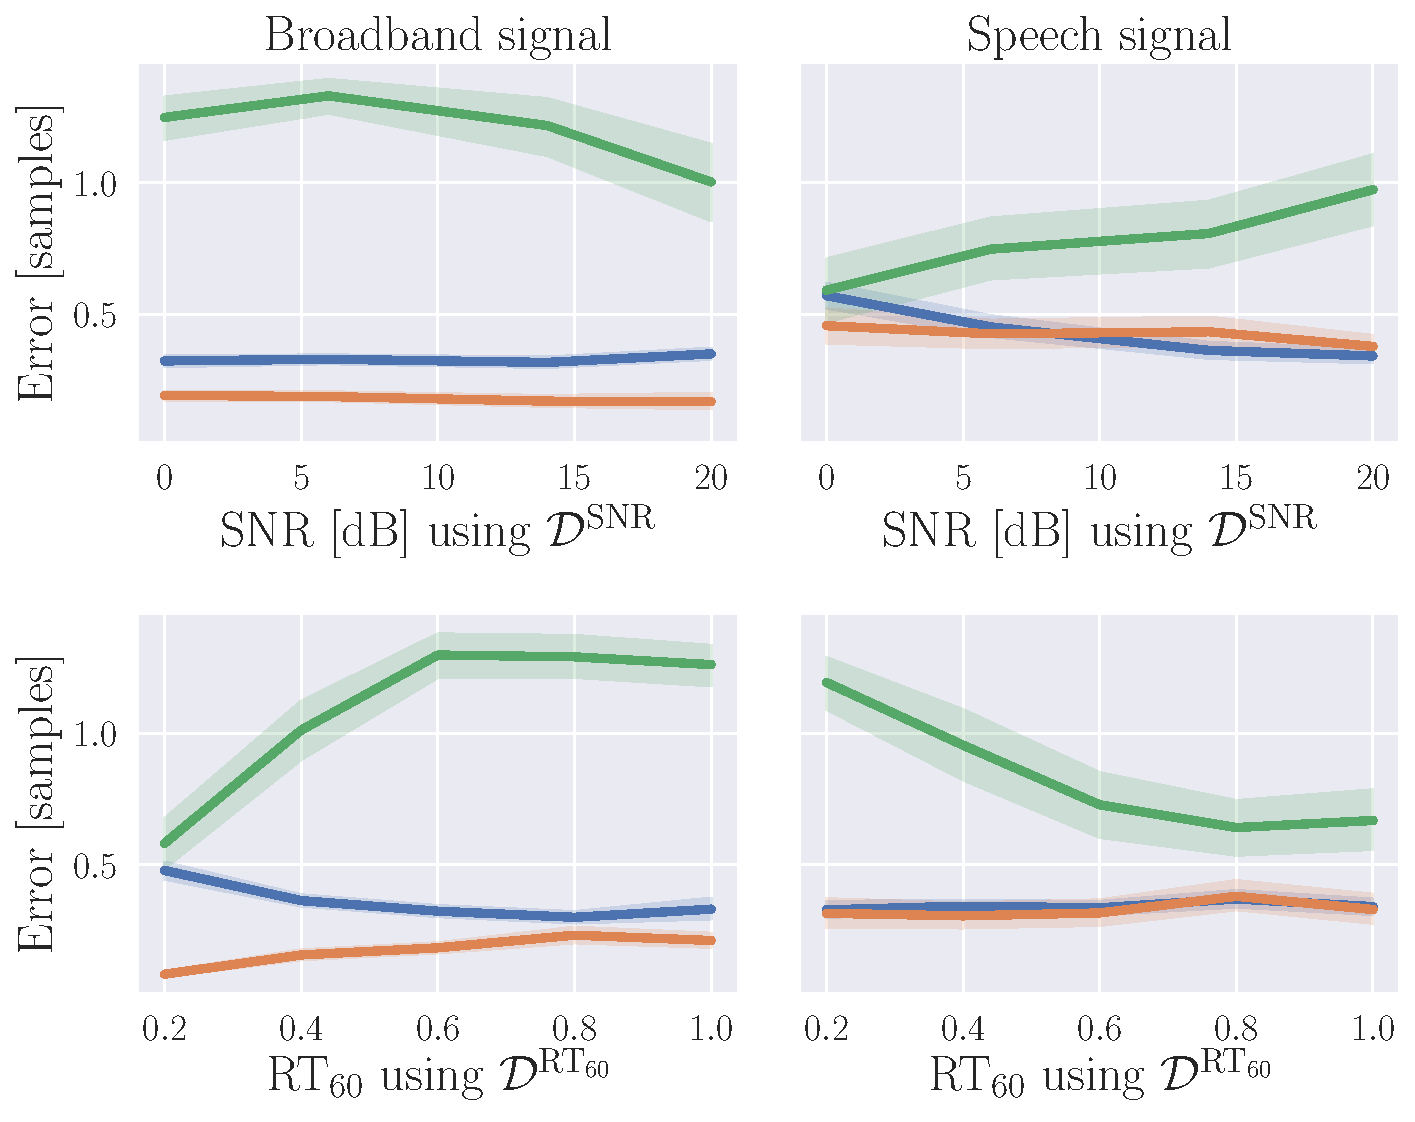
\includegraphics[width=.49\textwidth]{figures/blaster/e_k-7_thr-2_bns_crocco_blaster.pdf}
    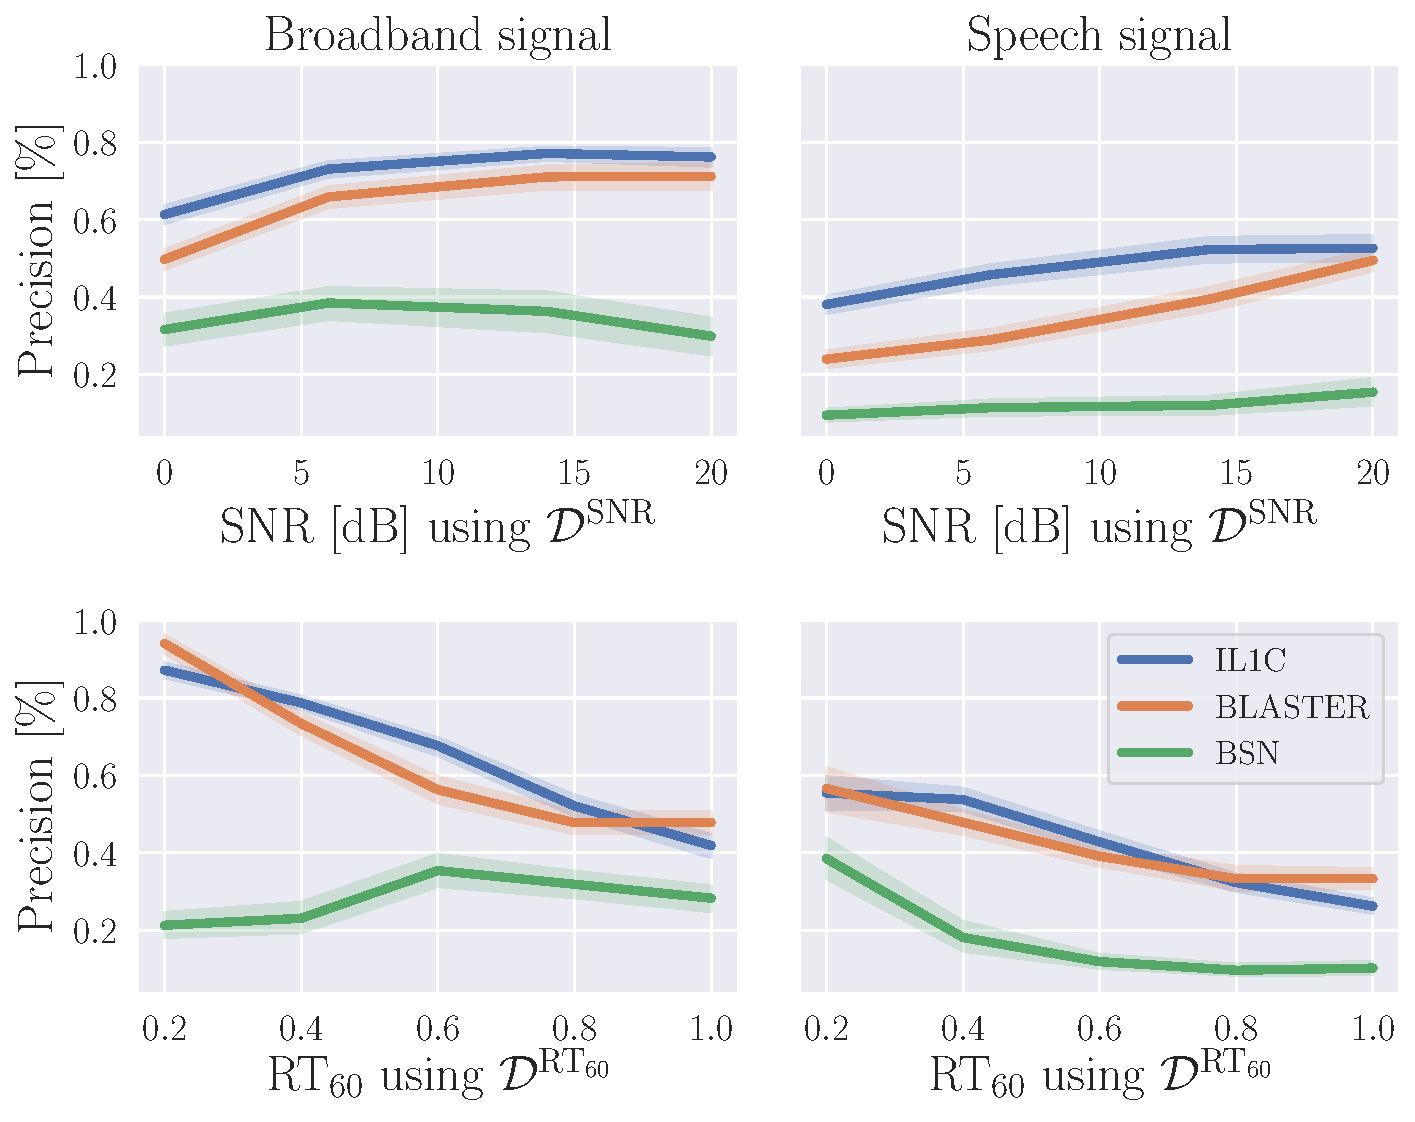
\includegraphics[width=.49\textwidth]{figures/blaster/p_k-7_thr-2_bns_crocco_blaster.pdf}

    \vspace*{2pt}
    \begin{center}
    \caption{%
        \label{fig:error_precision_snr_rt}
        Line plot with error bands for error (left) and precision (right) versus SNR level (top) and \RT{} level (bottom) using broadband and speech signals for the task of recovering $R=7$ echoes. A threshold of $\tau_{\textrm{max}}=2$ samples is used to compute the precision.
    }
    \end{center}
\vspace{-3mm}
\end{figure*}

The proposed method (\algoBraire) is compared against the non-negative $\ell_1$-norm method (\algoBsn) of~\cite{Lin2007} and the iterative $\ell_1$-norm approach (\algoCrocco) described in~\cite{Crocco2016}.
The problem is formulated as estimating the time location of the first $R=7$ strongest components of the RIRs for 2 microphones listening to a single sound source in a shoebox room. It corresponds to the challenging task of estimating
%all the
first-order early reflections.
The robustness of the methods is tested against different level of noise (SNR) and reverberation time (\RT{}).

We propose to compute a \textit{path of solutions} to automatically estimate the regularization parameter $\lambda$  in~\eqref{eq:TV-BLASSO}.
More precisely, let $\lambda_{\max}$ be the smallest value of $\lambda$ such that the null measure is the solution to~\eqref{eq:TV-BLASSO}.
It can be shown that $\lambda_{\max}$ is upper bounded by $\max_{\theta\in\Theta} \kvbar{\bfy^\intercal\opObs\delta_\theta}$.
Starting from $\ell=1$ and the empty filter, we consider a sequential implementation where the solution of~\eqref{eq:TV-BLASSO} is computed for $\lambda_\ell= 10^{-0.05\ell}\lambda_{\max}$ until the desired number of spikes is found in each channel when incrementing $\ell$.
For each $\lambda_\ell$, we search for a solution of~\eqref{eq:TV-BLASSO} with the solution obtained for $\lambda_{\ell-1}$ as a warm start.

The quality of the AER estimation is assessed in terms of precision\footnote{Since only $K$ time locations are considered in both the ground truth and the estimation, precision and recall are equal.} in percentage as in the literature of onset detection~\cite{Bock2012} and the root-mean-square-error (RMSE) in samples.
Both metrics evaluate only the \textit{matched} peaks, where a \textit{match} is defined as being within a small window $\thr$ of a reference delay. These two metrics are similar to the ones used in~\cite{Crocco2015}.

For this purpose we created three synthetic datasets of $1000$ observations each:
%As summarized in Table~\ref{tab:datasets},
\dsetValid{} is used for tuning the hyperparameter $\lambda$ and the peak-picking parameters for \algoCrocco{} and \algoBsn{} using \RT{} and SNR randomly drawn from $\mathcal{U}[0, 1]$ (sec) and $\mathcal{U}[0, 20]$ (dB) respectively; \dsetSNR{} features SNR value uniformly sampled in $[0, 6, 14, 20, \infty]$ while the \RT{} is kept fixed to $400$ ms; akin the \dsetRT{} is built sampling \RT{} value uniformly in $[200, 400, 600, 800, 1000]$ ms keeping SNR fix to 20 dB.
Moreover, while for \dsetValid{} broadband signals (white noise) are used as the source, for \dsetSNR{} and \dsetRT{} speech utterances from the TIMIT dataset are also included.
The signal duration is kept fixed to 1 s with sampling frequency $\Fs = 16$ kHz.

For a given \RT{} value and room with random dimensions, a unique absorption coefficient is assigned to all surfaces based on the Sabine's formula. Then, the two microphones and the source are randomly positioned inside the room. The parameters of such audio scene are then passed as input to the \texttt{pyroomacoustic} simulator~\cite{Scheibler_2018}, which returns the corresponding RIRs as well as the \textit{off-grid} echo delays and attenuation coefficients computed with the Image Method~\cite{Allen1979}.
Note that when generating the data, no samples have been pruned to match any minimal separation condition.

To generate the microphone signals, an oversampled version of the source signal is convolved with ideal RIRs at high frequency ($\Fs=1024$ kHz) made up of on-grid Dirac\textit{s}. The results are later resampled to meet the original $\Fs$ and Gaussian white noise is added to meet the given SNR value.

\begin{table}[ht]
    \centering
    %\begin{table}[t]
    {
        \centering
        \begin{tabular}{lccccc|ccccc}
        \toprule
               & \multicolumn{10}{c}{Precision [\%]}	\\
               \cline{2-11}
               & \multicolumn{5}{c|}{R = 2 echoes} & \multicolumn{5}{c}{R = 7 echoes} \\
               %
               \hline
               %
    $\thr$ & $0.5$ & $1$ & $2$ & $3$ & $10$ & $0.5$ & $1$ & $2$ & $3$ & $10$ \\ \hline
    BSN &  8 &           9 &          27 &          46 &           62 &           5 &           8 &          38 &          54 &  {73}  \\
    IL1C &           51 &          55 &          55 &          56 &           58 &          42 &          53 &          55 &          56 &         58 \\
    BLASTER & \textbf{68}  & \textbf{73}  & \textbf{74}  & \textbf{75}  & \textbf{75}   &{46}  &          53 &  {56}& {57} &         61 \\
    \bottomrule
    \end{tabular}
    }
    %\end{table*}


    % %\begin{table*}[t]
    % {
    %     \centering
    %     \scriptsize
    %     \begin{tabular}{lcccccccccc|ccccc|ccccc}
    %     \toprule
    %            & \multicolumn{10}{c|}{Error [samples]}                                                                                               & \multicolumn{10}{c}{Precision [\%]}                                                                           \\ \cline{2-21}
    %            & \multicolumn{5}{c|}{K = 2 echoes}                                           & \multicolumn{5}{c|}{K = 7 echoes}                     & \multicolumn{5}{c|}{K = 2 echoes}                     & \multicolumn{5}{c}{K = 7 echoes}                     \\ \hline
    % $\thr$ & $0.5$ & $1$ & $2$ & $3$ & \multicolumn{1}{c|}{$10$} & $0.5$ & $1$ & $2$ & $3$ & $10$ & $0.5$ & $1$ & $2$ & $3$ & $10$ & $0.5$ & $1$ & $2$ & $3$ & $10$ \\ \hline
    % \algoBsn &  \textbf{0.01} &\textbf{0.05}&        1.07 &        1.53 &\multicolumn{1}{c|}{2.85}         &\textbf{0.05}&        0.24 &        1.19 &        1.53 &         3.09 &           8 &           9 &          27 &          46 &           62 &           5 &           8 &          38 &          54 & \textbf{73}  \\
    % \algoCrocco &        0.20 &        0.23 &        0.24 &        0.26 &\multicolumn{1}{c|}{0.40}         &        0.20 &        0.28 &        0.33 &\textbf{0.37}&\textbf{0.83} &          51 &          55 &          55 &          56 &           58 &          42 &          53 &          55 &          56 &         58 \\
    % \algoBraire &        0.06 &        0.10 &\textbf{0.14}&\textbf{0.20}&\multicolumn{1}{c|}{\textbf{0.34}}&        0.13 &\textbf{0.20}&\textbf{0.32}&        0.42 &         1.48 &\textbf{68}  &\textbf{73}  &\textbf{74}  &\textbf{75}  &\textbf{75}   &\textbf{46}  &          53 &  \textbf{56}& \textbf{57} &         61 \\
    % \bottomrule
    % \end{tabular}
    % }
    %\end{table}
    \caption{\label{tab:error_precision_thr} Precision for different threshold $\thr$ in samples for the recovery of $R = 2$ and $7$ echoes, \RT{} = $200$ ms and SNR = 20 dB.}
\end{table}

\begin{figure}[t!]
    \centering
        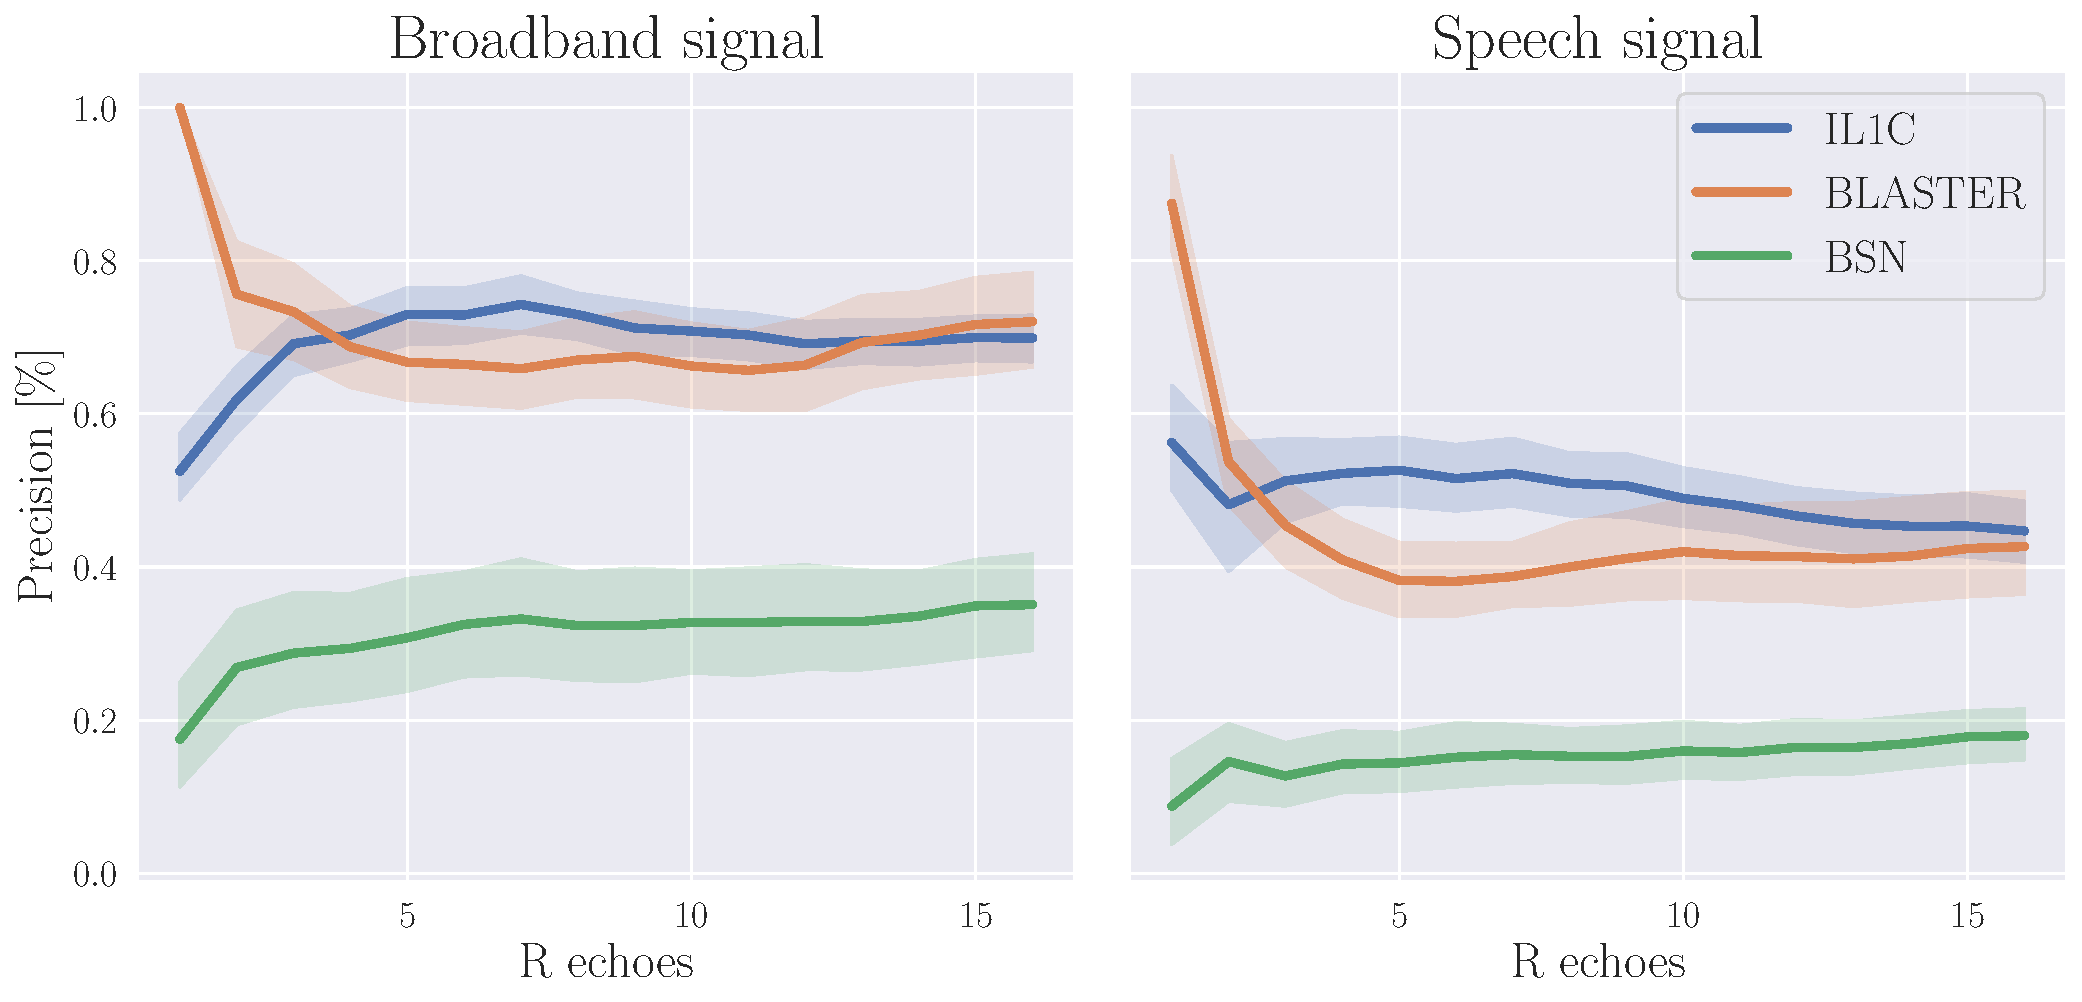
\includegraphics[width=\linewidth]{figures/blaster/p_k-7_thr-2_bns_crocco_blaster-peak_withRechoes.pdf}
        \caption{\label{fig:error_precision_kecho}  Line plots with error bands of precision versus number of echoes $R$ to be retrieved for broadband (left) and speech (right) signals with \RT{} = $400$ ms and SNR = 20 dB.}
\end{figure}

Quantitative results are reported in Fig.~\ref{fig:error_precision_snr_rt}, Fig.~\ref{fig:error_precision_kecho} and Tab.~\ref{tab:error_precision_thr}. Here, for both RMSE and Precision and for both broadband and speech signal, the metrics are displayed against the dataset parameters. We observe that \algoBsn{} performs worst in all tested conditions, possibly due to its strong reliance on the peak picking step. For $R=7$ or higher, \algoBraire{} yields similar or slightly worse performance than \algoCrocco{} for the considered noise and reverberation levels, with decreasing performance for both as these levels increase. Using speech rather than broadband signals also yields worse results for all methods. However, the echo timing RMSE is significantly smaller using \algoBraire{} due to its off-grid advantage. We also note that \algoBraire{} significantly outperforms \algoCrocco{} on the task of recovering $R=2$ echoes. As showed in Tab.~\ref{tab:error_precision_thr}, in mild conditions, up to 68\% of echoes can be retrieved by \algoBraire{} with errors lower than half a sample in that case. This is promising since the practical advantage of knowing the timing of two echoes per channel has been demonstrated in~\cite{DiCarlo2019,Scheibler2017}.